\documentclass{beamer}

\usepackage[utf8]{inputenc}
\usepackage[T1]{fontenc}
\usepackage{lmodern,tgadventor}
\usepackage{textcomp}
\usepackage{tikz}
\usetikzlibrary{backgrounds,decorations.text,fadings,trees}

\useinnertheme{rectangles}
\usecolortheme[accent=red]{solarized}
\setbeamercolor{description item}{fg=solarizedAccent}
\beamertemplatenavigationsymbolsempty
\setbeamertemplate{footline}[frame number]

% Shell highlighting
\newcommand{\command}[1]{\textcolor{solarizedAccent}{\$}
                         \textcolor{solarizedRebase2}{#1}}
\newcommand{\comment}[1]{\textit{\# #1}}
\newcommand{\hiRed}[1]{\textcolor{solarizedRed}{#1}}
\newcommand{\hiGreen}[1]{\textcolor{solarizedGreen}{#1}}
\newcommand{\hiBlue}[1]{\textcolor{solarizedBlue}{#1}}

% DAG commands
\newcommand\commit[2]{\node[commit] (#1) {};%
                      \node[clabel] (#1 label) at (#1) {\texttt{#1}: #2};}
\newcommand\ghost[1]{\coordinate (#1);}
\newcommand\connect[2]{\path[connections] (#1) to[out=90,in=-90] (#2);}
\newcommand\gittag[1]{%
 \begin{tikzpicture}[baseline]
  \node[fill=solarizedRebase02, rounded corners, inner sep=1pt, anchor=base] {
    \color{solarizedYellow}\vphantom{|}#1
   };
 \end{tikzpicture}%
}
\newcommand\branch[1]{%
 \begin{tikzpicture}[baseline]
  \node[fill=solarizedRebase02, rounded corners, inner sep=1pt, anchor=base] {
    \color{solarizedRed}\vphantom{|}#1
   };
 \end{tikzpicture}%
}

% http://tex.stackexchange.com/questions/55806/tikzpicture-in-beamer/55827#55827
\tikzset{
  invisible/.style={opacity=0},
  visible on/.style={alt=#1{}{invisible}},
  alt/.code args={<#1>#2#3}{%
    \alt<#1>{\pgfkeysalso{#2}}{\pgfkeysalso{#3}}
  },
}

\author{Elliott Sales de Andrade}
\title{CIG Seismo Code on Git/GitHub}
\institute{University of Toronto}
\titlegraphic{%
 \begin{tikzpicture}[
    commit/.style={draw, circle, fill=solarizedViolet, inner sep=0pt,
                   minimum size=5pt},
    clabel/.style={right, outer sep=1em},
    connections/.style={draw, solarizedViolet}
  ]
  \useasboundingbox (-1,1em) rectangle (1,8em); % Mysteriously chosen to fit...
  \matrix [column sep={1em,between origins}, row sep=\lineskip,
           ampersand replacement=\&]%
  {
   \commit{cd83b68}{\gittag{v6.0.0} \branch{master} submodules updated} \& \& \\
   \commit{170e5f7}{Update submodules in master} \& \& \\
   \commit{c0bc5ba}{Merge remote-tracking branch `origin/devel'} \& \& \\
   \& \commit{754300e}{Update README.md} \& \\
   \& \commit{40bcfdd}{Merge pull request \#68 from QuLogic/readme} \& \\
   \& \& \commit{e2f2928}{section-ify readme file.} \\
   \& \& \commit{eb6066e}{change to markdown so github linkifies stuff.} \\
   \& \& \commit{5babcb0}{add links to submodules in readme.} \\
   \& \commit{2b70a18}{merge pull request \#67 from komatits/devel} \& \\
   \ghost{5e338b5} \& \& \\
  };
  \connect{170e5f7}{cd83b68};
  \connect{c0bc5ba}{170e5f7};
  \connect{754300e}{c0bc5ba};
  \connect{40bcfdd}{754300e};
  \connect{e2f2928}{40bcfdd};
  \connect{eb6066e}{e2f2928};
  \connect{5babcb0}{eb6066e};
  \connect{2b70a18}{5babcb0};
  \connect{2b70a18}{40bcfdd};
  \connect{5e338b5}{2b70a18};
  \connect{5e338b5}{c0bc5ba};
  \fill [color=solarizedRebase03, path fading=north] (-6,-1.1) rectangle (6,.8);
 \end{tikzpicture}%
}

\begin{document}

\begin{frame}[plain,noframenumbering]
 \titlepage
\end{frame}

\begin{frame}
 \frametitle{Outline}
 \tableofcontents
\end{frame}

\section{Introduction}

\begin{frame}
 \frametitle{Introduction}

 \begin{itemize}
  \item CIG is transitioning code from Subversion to Git
  \item Also shifting most hosting to \href{https://github.com/}{GitHub}
  \item All Seismology code has been migrated:
   \begin{itemize}
    \item \href{https://github.com/geodynamics/specfem1d}{Specfem1D}
    \item \href{https://github.com/geodynamics/specfem2d}{Specfem2D}
    \item \href{https://github.com/geodynamics/specfem3d}{Specfem3D}
    \item \href{https://github.com/geodynamics/specfem3d_globe}{Specfem3D Globe}
    \item \href{https://github.com/geodynamics/mineos}{Mineos}
    \item \href{https://github.com/geodynamics/flexwin}{Flexwin}
    \item \href{https://github.com/geodynamics/axisem}{AxiSEM}
   \end{itemize}
  \item Also code for
        \href{http://geodynamics.org/cig/software/\#cs}{Computational Science},
        \href{http://geodynamics.org/cig/software/\#geodyn}{Geodynamo},
        \href{http://geodynamics.org/cig/software/\#long}{Long-Term Tectonics},
        \href{http://geodynamics.org/cig/software/\#mc}{Mantle Convection},
        \href{http://geodynamics.org/cig/software/\#short}{Short-Term Crustal
        Dynamics}
 \end{itemize}
\end{frame}

\subsection{What is Git?}

\begin{frame}
 \frametitle{Introduction}
 \framesubtitle{What is Git?}

 The stupid content tracker\footnotemark
 \begin{itemize}
  \item \href{http://git-scm.com/about/distributed}{Distributed}
   \begin{itemize}
    \item Multiple backups
    \item Flexible workflow
   \end{itemize}
  \item \href{http://git-scm.com/about/branching-and-merging}{Quick and easy
        branching}
   \begin{itemize}
    \item Frictionless context switching
    \item Role-based codelines
    \item Feature based workflow
    \item Disposable experimentation
   \end{itemize}
  \item \href{http://git-scm.com/about/small-and-fast}{Small and fast}
        --- One or two orders of magnitude faster than SVN (except cloning)
  \item \href{http://git-scm.com/about/info-assurance}{Repository integrity}
        --- Files, commit messages, dates
  \item \href{http://git-scm.com/about/staging-area}{Staging area}
        --- Flexible committing
  \item \href{http://git-scm.com/about/free-and-open-source}{Free and open
        source} --- GNU GPL 2.0
 \end{itemize}

 \footnotetext{\url{http://git-scm.com/about/}}
\end{frame}

\subsection{What is GitHub?}

\begin{frame}
 \frametitle{Introduction}
 \framesubtitle{What is GitHub?}

 Provides hosting and resources for open source software:
 \begin{itemize}
  \item Issue tracking
   \begin{itemize}
    \item Tasks
    \item Features
    \item Pull requests
    \item etc.
   \end{itemize}
  \item Code review
   \begin{itemize}
    \item Commit comments,
    \item Pull requests,
    \item Diffs,
    \item etc.
   \end{itemize}
  \item Wikis
  \item Collaborative tools
  \item Statistics
 \end{itemize}
\end{frame}

\subsection{Version Control Basics}

\begin{frame}
 \frametitle{Version Control Concepts}

 \begin{description}[Operations]
  \item[Repository] Complete copy of entire history of project\\
                    Files, Changes, Author names, Dates, etc.
  \item[Commit] Atomic record of changes to files, Author (and committer) of
                change, Date
  \item[Branch] Name for a commit that follows new commits (e.g.,
                amazing-new-feature)
  \item[Tag] Immovable name for a commit (e.g., v1.0)
  \item[Operations]
   \begin{itemize}
    \item Clone --- Download a copy of history
    \item Commit --- Record your changes
    \item Fetch --- Download new changes
    \item Merge --- Combine new changes with existing files
    \item \ldots
   \end{itemize}
 \end{description}
\end{frame}

\begin{frame}
 \frametitle{Version Control Concepts with Subversion}

 \vfill
 \begin{center}
  {\LARGE \alert{Ignore} Subversion if possible} \\
  {\small (Next three slides for those who know it already)}
 \end{center}
 \vfill
\end{frame}

%
% SVN Checkout
%

\begin{frame}
 \frametitle{Version Control Concepts with Subversion}
 \framesubtitle{Checkout}

 \begin{columns}
  \begin{column}{0.3\textwidth}
   \begin{tikzpicture}[
      remember picture,
      show background rectangle,
      commit/.style={draw, rectangle, rounded corners, fill=solarizedRebase02,
                     inner sep=1pt, minimum width=1.5em},
      connections/.style={draw}
    ]
    \matrix [column sep={1em,between origins}, row sep={1.5em,between origins},
             ampersand replacement=\&]%
    {
     \ghost{name}; \\
     \ghost{10}; \\
     \node[commit, visible on=<3->] (9) {9}; \\
     \node[commit, visible on=<3->] (8) {8}; \\
     \node[commit] (7) {7}; \\
     \node[commit] (6) {6}; \\
     \node[commit] (5) {5}; \\
     \node[commit] (4) {4}; \\
     \node[commit] (3) {3}; \\
     \node[commit] (2) {2}; \\
     \ghost{1}; \\
    };
    \node[anchor=south, align=center] at (name) {Central\\Repository};
    \foreach \x in {3,...,7} {
     \pgfmathparse{int(\x-1)}
     \connect{\pgfmathresult}{\x};
    }
    \path[connections, densely dashed] (1) -- (2);
    \path[connections, visible on=<3->] (7) -- (8);
    \path[connections, visible on=<3->] (8) -- (9);
   \end{tikzpicture}
  \end{column}
  \begin{column}{0.6\textwidth}
   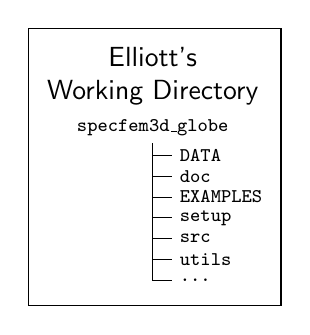
\begin{tikzpicture}[%
      remember picture,
      show background rectangle,
      background rectangle/.style={draw, visible on=<4->},
      visible on=<4->,
      every node/.style={anchor=west, minimum height=1em,
                         font={\scriptsize\ttfamily}, inner sep=2.5pt},
      every edge/.style={thick},
      root/.style={},
      grow via three points={one child at (0.25,-1em) and
                             two children at (0.25,-1em) and (0.25,-1.75em)},
      edge from parent path={(\tikzparentnode.south) |- (\tikzchildnode.west)}
    ]
    \node [root] (E root) {specfem3d\_globe}
     child { node {DATA} }
     child { node {doc} }
     child { node {EXAMPLES} }
     child { node {setup} }
     child { node {src} }
     child { node {utils} }
     child { node {\dots} };
    \node[anchor=south, font={\sffamily}, align=center] at (E root.north)
     {Elliott's\\Working Directory};
   \end{tikzpicture}

   \hfill
   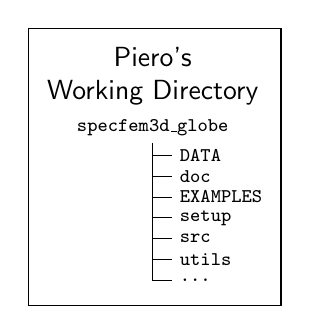
\begin{tikzpicture}[%
      remember picture,
      show background rectangle,
      background rectangle/.style={draw, visible on=<2->},
      visible on=<2->,
      every node/.style={anchor=west, minimum height=1em,
                         font={\scriptsize\ttfamily}, inner sep=2.5pt},
      every edge/.style={thick},
      root/.style={},
      grow via three points={one child at (0.25,-1em) and
                             two children at (0.25,-1em) and (0.25,-1.75em)},
      edge from parent path={(\tikzparentnode.south) |- (\tikzchildnode.west)}
    ]
    \node [root] (P root) {specfem3d\_globe}
     child { node {DATA} }
     child { node {doc} }
     child { node {EXAMPLES} }
     child { node {setup} }
     child { node {src} }
     child { node {utils} }
     child { node {\dots} };
    \node[anchor=south, font={\sffamily}, align=center] at (P root.north)
     {Piero's\\Working Directory};
   \end{tikzpicture}
  \end{column}
 \end{columns}

 \begin{tikzpicture}[
    remember picture, overlay,
    path/.style={thick, ->},
    label/.style={decorate, decoration={text along path, text align=center,
                                        text color=solarizedRebase0,
                                        raise=1pt,
                                        text={svn checkout}}}
  ]
  \draw<2>[path] (7.east) to[out=0,in=180] (P root.west);
  \draw<2>[label] (7.east) to[out=0,in=180] (P root.west);
  \draw<3->[path] (P root.west) to[out=180,in=0] (7.east);
  \draw<4->[path] (9.east) to[out=0,in=180] (E root.west);
  \draw<4->[label] (9.east) to[out=0,in=180] (E root.west);
 \end{tikzpicture}
\end{frame}

%
% SVN Commit
%

\begin{frame}
 \frametitle{Version Control Concepts with Subversion}
 \framesubtitle{Commits}

 \begin{columns}
  \begin{column}{0.3\textwidth}
   \begin{tikzpicture}[
      remember picture,
      show background rectangle,
      commit/.style={draw, rectangle, rounded corners, fill=solarizedRebase02,
                     inner sep=1pt, minimum width=1.5em},
      connections/.style={draw}
    ]
    \matrix [column sep={1em,between origins}, row sep={1.5em,between origins},
             ampersand replacement=\&]%
    {
     \ghost{name}; \\
     \node[commit, visible on=<3->] (10) {10}; \\
     \node[commit] (9) {9}; \\
     \node[commit] (8) {8}; \\
     \node[commit] (7) {7}; \\
     \node[commit] (6) {6}; \\
     \node[commit] (5) {5}; \\
     \node[commit] (4) {4}; \\
     \node[commit] (3) {3}; \\
     \node[commit] (2) {2}; \\
     \ghost{1}; \\
    };
    \node[anchor=south, align=center] at (name) {Central\\Repository};
    \foreach \x in {3,...,9} {
     \pgfmathparse{int(\x-1)}
     \connect{\pgfmathresult}{\x};
    }
    \path[connections, densely dashed] (1) -- (2);
    \path[connections, visible on=<3->] (9) -- (10);
   \end{tikzpicture}
  \end{column}
  \begin{column}{0.6\textwidth}
   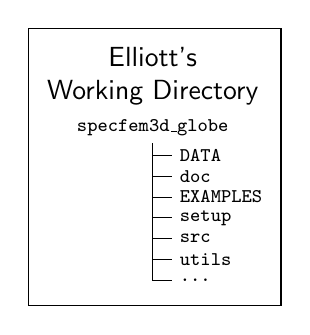
\begin{tikzpicture}[%
      remember picture,
      show background rectangle,
      every node/.style={anchor=west, minimum height=1em,
                         font={\scriptsize\ttfamily}, inner sep=2.5pt},
      every edge/.style={thick},
      root/.style={},
      grow via three points={one child at (0.25,-1em) and
                             two children at (0.25,-1em) and (0.25,-1.75em)},
      edge from parent path={(\tikzparentnode.south) |- (\tikzchildnode.west)}
    ]
    \node [root] (E root) {specfem3d\_globe}
     child { node {DATA} }
     child { node {doc} }
     child { node {EXAMPLES} }
     child { node {setup} }
     child { node {src} }
     child { node {utils} }
     child { node {\dots} };
    \node[anchor=south, font={\sffamily}, align=center] at (E root.north)
     {Elliott's\\Working Directory};
   \end{tikzpicture}

   \hfill
   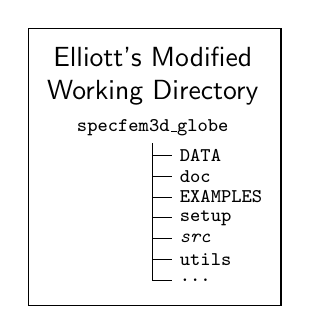
\begin{tikzpicture}[%
      remember picture,
      show background rectangle,
      background rectangle/.style={draw,visible on=<2-3>},
      visible on=<2-3>,
      every node/.style={anchor=west, minimum height=1em,
                         font={\scriptsize\ttfamily}, inner sep=2.5pt},
      every edge/.style={thick},
      root/.style={},
      grow via three points={one child at (0.25,-1em) and
                             two children at (0.25,-1em) and (0.25,-1.75em)},
      edge from parent path={(\tikzparentnode.south) |- (\tikzchildnode.west)}
    ]
    \node [root] (M root) {specfem3d\_globe}
     child { node {DATA} }
     child { node {doc} }
     child { node {EXAMPLES} }
     child { node {setup} }
     child { node {\itshape src} }
     child { node {utils} }
     child { node {\dots} };
    \node[anchor=south, font={\sffamily}, align=center] at (M root.north)
     {Elliott's Modified\\Working Directory};
   \end{tikzpicture}
  \end{column}
 \end{columns}

 \begin{tikzpicture}[
    remember picture, overlay,
    path/.style={thick, ->},
    label/.style={decorate, decoration={text along path, text align=center,
                                        text color=solarizedRebase0}}
  ]
  \draw<1-2>[path] (E root.west) to[out=180,in=0] (9.east);
  \draw<2-3>[path] (E root.east) to[out=0,in=0] (M root.east);
  \draw<2>[label, decoration={raise=1pt, text={Editing}}]
   (E root.east) to[out=0,in=0] (M root.east);
  \draw<3>[path, dashed] (E root.west) to[out=180,in=0] (9.east);
  \draw<3>[path] (M root.west) to[out=180,in=0] (10.east);
  \draw<3>[label, decoration={raise=-1em, text={svn commit}}]
   (10.east) to[out=0,in=180] (M root.west);
  \draw<4->[path] (E root.west) to[out=180,in=0] (10.east);
 \end{tikzpicture}
\end{frame}

%
% SVN Update
%

\begin{frame}
 \frametitle{Version Control Concepts with Subversion}
 \framesubtitle{Updating}

 \begin{columns}
  \begin{column}{0.3\textwidth}
   \begin{tikzpicture}[
      remember picture,
      show background rectangle,
      commit/.style={draw, rectangle, rounded corners, fill=solarizedRebase02,
                     inner sep=1pt, minimum width=1.5em},
      connections/.style={draw}
    ]
    \matrix [column sep={1em,between origins}, row sep={1.5em,between origins},
             ampersand replacement=\&]%
    {
     \ghost{name}; \\
     \node[commit] (10) {10}; \\
     \node[commit] (9) {9}; \\
     \node[commit] (8) {8}; \\
     \node[commit] (7) {7}; \\
     \node[commit] (6) {6}; \\
     \node[commit] (5) {5}; \\
     \node[commit] (4) {4}; \\
     \node[commit] (3) {3}; \\
     \node[commit] (2) {2}; \\
     \ghost{1}; \\
    };
    \node[anchor=south, align=center] at (name) {Central\\Repository};
    \foreach \x in {3,...,10} {
     \pgfmathparse{int(\x-1)}
     \connect{\pgfmathresult}{\x};
    }
    \path[connections, densely dashed] (1) -- (2);
   \end{tikzpicture}
  \end{column}
  \begin{column}{0.6\textwidth}
   \vfill

   \hfill
   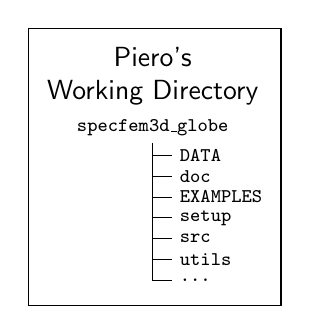
\begin{tikzpicture}[%
      remember picture,
      show background rectangle,
      every node/.style={anchor=west, minimum height=1em,
                         font={\scriptsize\ttfamily}, inner sep=2.5pt},
      every edge/.style={thick},
      root/.style={},
      grow via three points={one child at (0.25,-1em) and
                             two children at (0.25,-1em) and (0.25,-1.75em)},
      edge from parent path={(\tikzparentnode.south) |- (\tikzchildnode.west)}
    ]
    \node [root] (P root) {specfem3d\_globe}
     child { node {DATA} }
     child { node {doc} }
     child { node {EXAMPLES} }
     child { node {setup} }
     child { node {src} }
     child { node {utils} }
     child { node {\dots} };
    \node[anchor=south, font={\sffamily}, align=center] at (P root.north)
     {Piero's\\Working Directory};
   \end{tikzpicture}
  \end{column}
 \end{columns}

 \begin{tikzpicture}[
    remember picture, overlay,
    path/.style={thick, ->},
    label/.style={decorate, decoration={text along path, text align=center,
                                        text color=solarizedRebase0,
                                        raise=1pt,
                                        text={svn update}}}
  ]
  \draw<1>[path] (P root.west) to[out=180,in=0] (7.east);
  \draw<2>[path, dashed] (P root.west) to[out=180,in=0] (7.east);
  \draw<2>[path] (10.east) to[out=0,in=180] (P root.west);
  \draw<2>[label] (10.east) to[out=0,in=180] (P root.west);
  \draw<3>[path] (P root.west) to[out=180,in=0] (10.east);
 \end{tikzpicture}
\end{frame}

\begin{frame}
 \frametitle{Version Control Concepts with Git}

 \vfill
 \begin{center}
  {\LARGE \alert{Forget} Subversion if possible} \\
  {\small (Previous slides for those who know it already)}
 \end{center}
 \vfill
\end{frame}

%
% Git Cloning
%

\begin{frame}
 \frametitle{Version Control Concepts with Git}
 \framesubtitle{Cloning}

 \begin{columns}
  \begin{column}{0.3\textwidth}
   \begin{tikzpicture}[
     remember picture,
     show background rectangle,
     commit/.style={draw, rectangle, rounded corners, fill=solarizedRebase02,
                    inner sep=1pt, minimum width=1.5em},
     connections/.style={draw}
    ]
    \matrix [column sep={1em,between origins}, row sep={1.5em,between origins},
             ampersand replacement=\&]%
    {
     \ghost{name}; \\
     \ghost{10}; \\
     \node[commit, visible on=<3->] (9) {9}; \\
     \node[commit, visible on=<3->] (8) {8}; \\
     \node[commit] (7) {7}; \\
     \node[commit] (6) {6}; \\
     \node[commit] (5) {5}; \\
     \node[commit] (4) {4}; \\
     \node[commit] (3) {3}; \\
     \node[commit] (2) {2}; \\
     \ghost{1}; \\
    };
    \node[anchor=south, align=center] (repository) at (name)
     {Central\\Repository};
    \foreach \x in {3,...,7} {
     \pgfmathparse{int(\x-1)}
     \connect{\pgfmathresult}{\x};
    }
    \path[connections, densely dashed] (1) -- (2);
    \path[connections, visible on=<3->] (7) -- (8);
    \path[connections, visible on=<3->] (8) -- (9);
   \end{tikzpicture}
  \end{column}
  \begin{column}{0.6\textwidth}
   \begin{tikzpicture}[%
     remember picture,
     show background rectangle,
     background rectangle/.style={draw, visible on=<4->},
     visible on=<4->
    ]
    \begin{scope}[
      commit/.style={draw, circle, fill=solarizedRebase02,
                     inner sep=0.5pt, minimum width=0.5em,
                     font={\tiny\sffamily}},
      connections/.style={draw}
     ]
     \matrix [column sep={1em,between origins}, row sep={1em,between origins},
              ampersand replacement=\&]%
     {
      \node[commit] (E 9) {9}; \\
      \node[commit] (E 8) {8}; \\
      \node[commit] (E 7) {7}; \\
      \node[commit] (E 6) {6}; \\
      \node[commit] (E 5) {5}; \\
     };
     \node[anchor=south, align=center, font={\scriptsize}] at (E 9.north)
      (E repository) {Local\\Repository};
     \foreach \x in {6,...,9} {
      \pgfmathparse{int(\x-1)}
      \connect{E \pgfmathresult}{E \x};
     }
     \path[connections, densely dotted] (E 5.south) -- +(0,-0.5em);
    \end{scope}
    \begin{scope}[
      every node/.style={anchor=west, minimum height=1em,
                         font={\tiny\ttfamily}, inner sep=2.5pt},
      every edge/.style={thick},
      root/.style={},
      grow via three points={one child at (0.25,-0.75em) and
                             two children at (0.25,-.75em) and (0.25,-1.25em)},
      edge from parent path={(\tikzparentnode.south) |- (\tikzchildnode.west)}
     ]
     \node[anchor=west, font={\scriptsize\sffamily}, align=center, xshift=1em]
      at (E repository.east) (E work) {Working\\Directory};
     \node [root, anchor=north] at (E work.south) (E root) {specfem3d\_globe}
      child { node {DATA} }
      child { node {doc} }
      child { node {EXAMPLES} }
      child { node {setup} }
      child { node {src} }
      child { node {utils} }
      child { node {\dots} };
    \end{scope}
    \node[anchor=south, shift={(0.5em,1em)}] at (E repository.east)
     {Elliott's Computer};
    \draw[->] (E 9.east) to[out=0,in=180] (E root.west);
   \end{tikzpicture}

   \hfill
   \begin{tikzpicture}[%
     remember picture,
     show background rectangle,
     background rectangle/.style={draw, visible on=<2->},
     visible on=<2->
    ]
    \begin{scope}[
      commit/.style={draw, circle, fill=solarizedRebase02,
                     inner sep=0.5pt, minimum width=0.5em,
                     font={\tiny\sffamily}},
      connections/.style={draw}
     ]
     \matrix [column sep={1em,between origins}, row sep={1em,between origins},
              ampersand replacement=\&]%
     {
      \ghost{P 9}; \\
      \ghost{P 8}; \\
      \node[commit] (P 7) {7}; \\
      \node[commit] (P 6) {6}; \\
      \node[commit] (P 5) {5}; \\
     };
     \node[anchor=south, align=center, font={\scriptsize}] at (P 9.north)
      (P repository) {Local\\Repository};
     \foreach \x in {6,...,7} {
      \pgfmathparse{int(\x-1)}
      \connect{P \pgfmathresult}{P \x};
     }
     \path[connections, densely dotted] (P 5.south) -- +(0,-0.5em);
    \end{scope}
    \begin{scope}[
      every node/.style={anchor=west, minimum height=1em,
                         font={\tiny\ttfamily}, inner sep=2.5pt},
      every edge/.style={thick},
      root/.style={},
      grow via three points={one child at (0.25,-0.75em) and
                             two children at (0.25,-0.75em) and (0.25,-1.25em)},
      edge from parent path={(\tikzparentnode.south) |- (\tikzchildnode.west)}
     ]
     \node[anchor=west, font={\scriptsize\sffamily}, align=center, xshift=1em]
      at (P repository.east) (P work) {Working\\Directory};
     \node [root, anchor=north] at (P work.south) (P root) {specfem3d\_globe}
      child { node {DATA} }
      child { node {doc} }
      child { node {EXAMPLES} }
      child { node {setup} }
      child { node {src} }
      child { node {utils} }
      child { node {\dots} };
    \end{scope}
    \node[anchor=south, shift={(0.5em,1em)}] at (P repository.east)
     {Piero's Computer};
    \draw<2->[->] (P 7.east) to[out=0,in=180] (P root.west);
   \end{tikzpicture}
  \end{column}
 \end{columns}

 \begin{tikzpicture}[
   remember picture, overlay,
   path/.style={thick, ->},
   label/.style={decorate, decoration={text along path, text align=center,
                                       text color=solarizedRebase0,
                                       raise=1pt,
                                       text={git clone}}}
  ]
  \draw<2>[path] (repository) to[out=0,in=180] (P repository.west);
  \draw<2>[label] (repository) to[out=0,in=180] (P repository.west);
  \draw<3->[path,|-|] (repository) to[out=0,in=180] (P repository.west);
  \draw<4->[path] (repository) to[out=0,in=180] (E repository.west);
  \draw<4->[label] (repository) to[out=0,in=180] (E repository.west);
 \end{tikzpicture}
\end{frame}

%
% Git Commit
%

\begin{frame}
 \frametitle{Version Control Concepts with Git}
 \framesubtitle{Commits}

 \begin{columns}
  \begin{column}{0.3\textwidth}
   \begin{tikzpicture}[
     remember picture,
     show background rectangle,
     commit/.style={draw, rectangle, rounded corners, fill=solarizedRebase02,
                    inner sep=1pt, minimum width=1.5em},
     connections/.style={draw}
    ]
    \matrix [column sep={1em,between origins}, row sep={1.5em,between origins},
             ampersand replacement=\&]%
    {
     \ghost{name}; \\
     \node[commit, visible on=<5->] (10) {10}; \\
     \node[commit] (9) {9}; \\
     \node[commit] (8) {8}; \\
     \node[commit] (7) {7}; \\
     \node[commit] (6) {6}; \\
     \node[commit] (5) {5}; \\
     \node[commit] (4) {4}; \\
     \node[commit] (3) {3}; \\
     \node[commit] (2) {2}; \\
     \ghost{1}; \\
    };
    \node[anchor=south,align=center] (repository) at (name)
     {Central\\Repository};
    \foreach \x in {3,...,9} {
     \pgfmathparse{int(\x-1)}
     \connect{\pgfmathresult}{\x};
    }
    \path[connections, densely dashed] (1) -- (2);
    \path[connections, visible on=<5->] (9) -- (10);
   \end{tikzpicture}
  \end{column}
  \begin{column}{0.6\textwidth}
   \begin{tikzpicture}[%
      remember picture,
      show background rectangle
    ]
    \begin{scope}[
      commit/.style={draw, rectangle, rounded corners, fill=solarizedRebase02,
                     inner sep=1pt, minimum height=0.75em, minimum width=1em,
                     font={\tiny\sffamily}},
      connections/.style={draw}
     ]
     \matrix [column sep={1em,between origins}, row sep={1.2em,between origins},
              ampersand replacement=\&]%
     {
      \node[commit, visible on=<3->] (E 10) {10}; \\
      \node[commit] (E 9) {9}; \\
      \node[commit] (E 8) {8}; \\
      \node[commit] (E 7) {7}; \\
      \node[commit] (E 6) {6}; \\
      \node[commit] (E 5) {5}; \\
      \ghost{E 4}; \\
     };
     \node[anchor=south, align=center, font={\scriptsize}] at (E 10.north)
      (E repository) {Local\\Repository};
     \foreach \x in {6,...,9} {
      \pgfmathparse{int(\x-1)}
      \connect{E \pgfmathresult}{E \x};
     }
     \path[connections, densely dotted] (E 4) -- (E 5);
     \path[connections, visible on=<3->] (E 9) -- (E 10);
    \end{scope}
    \begin{scope}[
      every node/.style={anchor=west, minimum height=1em,
                         font={\tiny\ttfamily}, inner sep=2.5pt},
      every edge/.style={thick},
      root/.style={},
      grow via three points={one child at (0.25,-0.75em) and
                             two children at (0.25,-0.75em) and (0.25,-1.25em)},
      edge from parent path={(\tikzparentnode.south) |- (\tikzchildnode.west)}
     ]
     \node[anchor=west, font={\scriptsize\sffamily}, align=center, xshift=1em]
      at (E repository.east) (E work) {Working\\Directory};
     \node [root, anchor=north] at (E work.south) (E root) {specfem3d\_globe}
      child { node {DATA} }
      child { node {doc} }
      child { node {EXAMPLES} }
      child { node {setup} }
      child { node {src} }
      child { node {utils} }
      child { node (E last) {\dots} };
    \end{scope}
    \begin{scope}[
      visible on=<2-3>,
      every node/.style={anchor=west, minimum height=1em,
                         font={\tiny\ttfamily}, inner sep=2.5pt},
      every edge/.style={thick},
      root/.style={},
      label/.style={decorate, decoration={text along path, text align=center,
                                          text color=solarizedRebase0}},
      grow via three points={one child at (0.25,-0.75em) and
                             two children at (0.25,-0.75em) and (0.25,-1.25em)},
      edge from parent path={(\tikzparentnode.south) |- (\tikzchildnode.west)}
     ]
    \node[anchor=north, font={\scriptsize\sffamily}, align=center, xshift=1em]
     at (E last.south) (M work) {Modified\\Working Directory};
    \node [root, anchor=north] at (M work.south) (M root) {specfem3d\_globe}
     child { node {DATA} }
     child { node {doc} }
     child { node {EXAMPLES} }
     child { node {setup} }
     child { node {\itshape src} }
     child { node {utils} }
     child { node {\dots} };
    \end{scope}

    \draw<1-2>[->] (E root.west) to[out=180,in=0] (E 9.east);
    \draw<3>[->, dashed] (E root.west) to[out=180,in=0] (E 9.east);
    \draw<4->[->] (E root.west) to[out=180,in=0] (E 10.east);

    \node[anchor=south, shift={(1em,1em)}] at (E repository.east)
     {Elliott's Computer};
   \end{tikzpicture}
  \end{column}
 \end{columns}

 \begin{tikzpicture}[
    remember picture, overlay,
    path/.style={thick, ->},
    label/.style={decorate, decoration={text along path, text align=center,
                                        text color=solarizedRebase0}}
  ]
  \draw<1-4>[path,|-|] (repository.east) to[out=0,in=180] (E repository.west);
  \draw<2-3>[->] (E root.east) to[out=0,in=0] (M root.east);
  \draw<2>[label, decoration={raise=1pt,
                              text={|\scriptsize| Editing~~~~~}}]
   (E root.east) to[out=0,in=0] (M root.east);
  \draw<3>[->] (M root.west) to[out=180,in=0] (E 10.east);
  \draw<3>[label, decoration={raise=-0.75em,
                              text={|\scriptsize| git commit}}]
   (E 10.east) to[out=0,in=180] (M root.west);
  \draw<5>[path] (E repository.west) to[out=180,in=0] (repository.east);
  \draw<5>[label, decoration={raise=1pt, text={git push}}]
   (repository.east) to[out=0,in=180] (E repository.west);
 \end{tikzpicture}
\end{frame}

%
% Git Updating
%

\begin{frame}
 \frametitle{Version Control Concepts with Git}
 \framesubtitle{Updating}

 \begin{columns}
  \begin{column}{0.3\textwidth}
   \begin{tikzpicture}[
     remember picture,
     show background rectangle,
     commit/.style={draw, rectangle, rounded corners, fill=solarizedRebase02,
                    inner sep=1pt, minimum width=1.5em},
     connections/.style={draw}
    ]
    \matrix [column sep={1em,between origins}, row sep={1.5em,between origins},
             ampersand replacement=\&]%
    {
     \ghost{name}; \\
     \node[commit] (10) {10}; \\
     \node[commit] (9) {9}; \\
     \node[commit] (8) {8}; \\
     \node[commit] (7) {7}; \\
     \node[commit] (6) {6}; \\
     \node[commit] (5) {5}; \\
     \node[commit] (4) {4}; \\
     \node[commit] (3) {3}; \\
     \node[commit] (2) {2}; \\
     \ghost{1}; \\
    };
    \node[anchor=south, align=center] (repository) at (name)
     {Central\\Repository};
    \foreach \x in {3,...,10} {
     \pgfmathparse{int(\x-1)}
     \connect{\pgfmathresult}{\x};
    }
    \path[connections, densely dashed] (1) -- (2);
   \end{tikzpicture}
  \end{column}
  \begin{column}{0.6\textwidth}
   \vfill

   \hfill
   \begin{tikzpicture}[%
     remember picture,
     show background rectangle,
    ]
    \begin{scope}[
      commit/.style={draw, rectangle, rounded corners, fill=solarizedRebase02,
                     inner sep=1pt, minimum height=0.75em, minimum width=1em,
                     font={\tiny\sffamily}},
      connections/.style={draw}
     ]
     \matrix [column sep={1em,between origins}, row sep={1em,between origins},
              ampersand replacement=\&]%
     {
      \node[commit, visible on=<2->] (P 10) {10}; \\
      \node[commit, visible on=<2->] (P 9) {9}; \\
      \node[commit, visible on=<2->] (P 8) {8}; \\
      \node[commit] (P 7) {7}; \\
      \node[commit] (P 6) {6}; \\
      \node[commit] (P 5) {5}; \\
      \ghost{P 4}; \\
     };
     \node[anchor=south, align=center, font={\scriptsize}] at (P 10.north)
      (P repository) {Local\\Repository};
     \foreach \x in {6,...,7} {
      \pgfmathparse{int(\x-1)}
      \connect{P \pgfmathresult}{P \x};
     }
     \path[connections, densely dotted] (P 4) -- (P 5);
     \path[connections, visible on=<2->] (P 7) -- (P 8);
     \path[connections, visible on=<2->] (P 8) -- (P 9);
     \path[connections, visible on=<2->] (P 9) -- (P 10);
    \end{scope}
    \begin{scope}[
      every node/.style={anchor=west, minimum height=1em,
                         font={\tiny\ttfamily}, inner sep=2.5pt},
      every edge/.style={thick},
      root/.style={},
      grow via three points={one child at (0.25,-0.75em) and
                             two children at (0.25,-0.75em) and (0.25,-1.25em)},
      edge from parent path={(\tikzparentnode.south) |- (\tikzchildnode.west)}
     ]
     \node[anchor=west, font={\scriptsize\sffamily}, align=center, xshift=3em]
      at (P repository.east) (P work) {Working\\Directory};
     \node [root, anchor=north] at (P work.south) (P root) {specfem3d\_globe}
      child { node {DATA} }
      child { node {doc} }
      child { node {EXAMPLES} }
      child { node {setup} }
      child { node {src} }
      child { node {utils} }
      child { node {\dots} };
    \end{scope}
    \node[anchor=south, shift={(1.5em,1em)}] at (P repository.east)
     {Piero's Computer};

    \draw<1-2>[->] (P root.west) to[out=180,in=0] (P 7.east);
    \draw<3>[->, dashed] (P root.west) to[out=180,in=0] (P 7.east);
    \draw<3>[->] (P 10.east) to[out=0,in=180] (P root.west);
    \draw<4>[->] (P root.west) to[out=180,in=0] (P 10.east);
   \end{tikzpicture}
  \end{column}
 \end{columns}

 \begin{tikzpicture}[
   remember picture, overlay,
   path/.style={thick, ->},
   label/.style={decorate, decoration={text along path, text align=center,
                                       text color=solarizedRebase0, raise=1pt}}
  ]
  \draw<1>[path,|-|] (repository) to[out=0,in=180] (P repository.west);
  \draw<2>[path] (repository) to[out=0,in=180] (P repository.west);
  \draw<2>[label, decoration={text={git fetch}}]
   (repository) to[out=0,in=180] (P repository.west);
  \draw<3->[path,|-|] (repository) to[out=0,in=180] (P repository.west);
  \draw<3>[label, decoration={text={|\scriptsize| git merge}}]
   (P 10.east) to[out=0,in=180] (P root.west);
 \end{tikzpicture}
\end{frame}

\begin{frame}
 \frametitle{Git Basics}
 \framesubtitle{Commits}

 \begin{itemize}
  \item Denoted by SHA1 hash, e.g., cd83b686a7c6014e132933f685157d43151a665e
        (can be shortened); based on:
   \begin{itemize}
    \item Tree of files
    \item Parent commit(s)
    \item Commit message
    \item Author name/email/timestamp
    \item Committer name/email/timestamp
   \end{itemize}
  \pause
  \item Form a Directed Acyclic Graph, referenced by:
   \begin{itemize}
    \item Child commits
    \item Branches
    \item Tags
    \item HEAD (Working Directory link)
    \item The reflog (advanced, but useful at times)
   \end{itemize}
 \end{itemize}
\end{frame}

\begin{frame}
 \frametitle{Git Basics}
 \framesubtitle{Remotes}

 Remotes are references to other repositories; URIs can be:
 \begin{itemize}
  \item HTTPS:\\
    {\small \url{https://github.com/geodynamics/specfem3d_globe.git}}
  \item SSH:\\
    \url{git@github.com:geodynamics/specfem3d_globe.git}
  \item File:\\
    \url{file:///path/to/specfem3d_globe}
  \item Local Path:\\
    \url{/home/elliott/specfem3d_globe}
 \end{itemize}
\end{frame}

\begin{frame}
 \frametitle{Git Basics}
 \framesubtitle{Remotes}

 \begin{columns}
  \begin{column}{0.3\textwidth}
   \begin{tikzpicture}[
     remember picture,
     show background rectangle,
     commit/.style={draw, rectangle, rounded corners, fill=solarizedRebase02,
                    inner sep=1pt, minimum width=1.5em},
     connections/.style={draw}
    ]
    \matrix [column sep={1em,between origins}, row sep={1.5em,between origins},
             ampersand replacement=\&]%
    {
     \ghost{name}; \\
     \ghost{10}; \\
     \node[commit] (9) {9}; \\
     \node[commit] (8) {8}; \\
     \node[commit] (7) {7}; \\
     \node[commit] (6) {6}; \\
     \node[commit] (5) {5}; \\
     \node[commit] (4) {4}; \\
     \node[commit] (3) {3}; \\
     \node[commit] (2) {2}; \\
     \ghost{1}; \\
    };
    \node[anchor=south, align=center] (repository) at (name)
     {Central\\Repository};
    \foreach \x in {3,...,9} {
     \pgfmathparse{int(\x-1)}
     \connect{\pgfmathresult}{\x};
    }
    \path[connections, densely dashed] (1) -- (2);
   \end{tikzpicture}
  \end{column}
  \begin{column}{0.6\textwidth}
   \begin{tikzpicture}[%
     remember picture,
     show background rectangle
    ]
    \begin{scope}[
      commit/.style={draw, circle, fill=solarizedRebase02,
                     inner sep=0.5pt, minimum width=0.5em,
                     font={\tiny\sffamily}},
      connections/.style={draw}
     ]
     \matrix [column sep={1em,between origins}, row sep={1em,between origins},
              ampersand replacement=\&]%
     {
      \node[commit] (E 9) {9}; \\
      \node[commit] (E 8) {8}; \\
      \node[commit] (E 7) {7}; \\
      \node[commit] (E 6) {6}; \\
      \node[commit] (E 5) {5}; \\
     };
     \node[anchor=south, align=center, font={\scriptsize}] at (E 9.north)
      (E repository) {Local\\Repository};
     \foreach \x in {6,...,9} {
      \pgfmathparse{int(\x-1)}
      \connect{E \pgfmathresult}{E \x};
     }
     \path[connections, densely dotted] (E 5.south) -- +(0,-0.5em);
    \end{scope}
    \begin{scope}[
      every node/.style={anchor=west, minimum height=1em,
                         font={\tiny\ttfamily}, inner sep=2.5pt},
      every edge/.style={thick},
      root/.style={},
      grow via three points={one child at (0.25,-0.75em) and
                             two children at (0.25,-.75em) and (0.25,-1.25em)},
      edge from parent path={(\tikzparentnode.south) |- (\tikzchildnode.west)}
     ]
     \node[anchor=west, font={\scriptsize\sffamily}, align=center, xshift=1em]
      at (E repository.east) (E work) {Working\\Directory};
     \node [root, anchor=north] at (E work.south) (E root) {specfem3d\_globe}
      child { node {DATA} }
      child { node {doc} }
      child { node {EXAMPLES} }
      child { node {setup} }
      child { node {src} }
      child { node {utils} }
      child { node {\dots} };
    \end{scope}
    \node[anchor=south, shift={(0.5em,1em)}] at (E repository.east)
     {Elliott's Computer};
    \draw[->] (E 9.east) to[out=0,in=180] (E root.west);
   \end{tikzpicture}

   \hfill
   \begin{tikzpicture}[%
     remember picture,
     show background rectangle
    ]
    \begin{scope}[
      commit/.style={draw, circle, fill=solarizedRebase02,
                     inner sep=0.5pt, minimum width=0.5em,
                     font={\tiny\sffamily}},
      connections/.style={draw}
     ]
     \matrix [column sep={1em,between origins}, row sep={1em,between origins},
              ampersand replacement=\&]%
     {
      \node[commit] (P 9) {9}; \\
      \node[commit] (P 8) {8}; \\
      \node[commit] (P 7) {7}; \\
      \node[commit] (P 6) {6}; \\
      \node[commit] (P 5) {5}; \\
     };
     \node[anchor=south, align=center, font={\scriptsize}] at (P 9.north)
      (P repository) {Local\\Repository};
     \foreach \x in {6,...,9} {
      \pgfmathparse{int(\x-1)}
      \connect{P \pgfmathresult}{P \x};
     }
     \path[connections, densely dotted] (P 5.south) -- +(0,-0.5em);
    \end{scope}
    \begin{scope}[
      every node/.style={anchor=west, minimum height=1em,
                         font={\tiny\ttfamily}, inner sep=2.5pt},
      every edge/.style={thick},
      root/.style={},
      grow via three points={one child at (0.25,-0.75em) and
                             two children at (0.25,-0.75em) and (0.25,-1.25em)},
      edge from parent path={(\tikzparentnode.south) |- (\tikzchildnode.west)}
     ]
     \node[anchor=west, font={\scriptsize\sffamily}, align=center, xshift=1em]
      at (P repository.east) (P work) {Working\\Directory};
     \node [root, anchor=north] at (P work.south) (P root) {specfem3d\_globe}
      child { node {DATA} }
      child { node {doc} }
      child { node {EXAMPLES} }
      child { node {setup} }
      child { node {src} }
      child { node {utils} }
      child { node {\dots} };
    \end{scope}
    \node[anchor=south, shift={(0.5em,1em)}] at (P repository.east)
     {Piero's Computer};
    \draw[->] (P 9.east) to[out=0,in=180] (P root.west);
   \end{tikzpicture}
  \end{column}
 \end{columns}

 \begin{tikzpicture}[
   remember picture, overlay,
   path/.style={thick, ->},
   label/.style={decorate, decoration={text along path, text align=center,
                                       text color=solarizedRebase0,
                                       raise=1pt,
                                       text={remote}}}
  ]
  \draw<1>[path] (P repository.west) to[out=180,in=0] (repository);
  \draw<1>[label] (repository) to[out=0,in=180] (P repository.west);
  \draw<1>[path] (E repository.west) to[out=180,in=0] (repository);
  \draw<1>[label] (repository) to[out=0,in=180] (E repository.west);
  \draw<2>[path,<->] (P repository.west) to[out=180,in=180] (E repository.west);
  \draw<2>[label, decoration={raise=-1em}]
   (E repository.west) to[out=180,in=180] (P repository.west);
 \end{tikzpicture}
\end{frame}

\begin{frame}[fragile]
 \frametitle{Git Basics}
 \framesubtitle{Configuration}

 \begin{block}{User Name}
  \begin{verbatim}
$ git config --global user.name 'User Name'
$ git config --global user.email 'email@example.com'
\end{verbatim}
 \end{block}
 \pause
 \begin{block}{Conveniences}
  \begin{verbatim}
$ git config --global color.ui auto
$ git config --global push.default simple
\end{verbatim}
 \end{block}
\end{frame}


\section{Using CIG Code from Git}

\begin{frame}[plain,noframenumbering]
 \vfill
 \begin{center}
  \LARGE \color{solarizedAccent} Using CIG Code from Git
 \end{center}
 \vfill
\end{frame}

\begin{frame}
 \frametitle{Using CIG Code from Git(Hub)}

 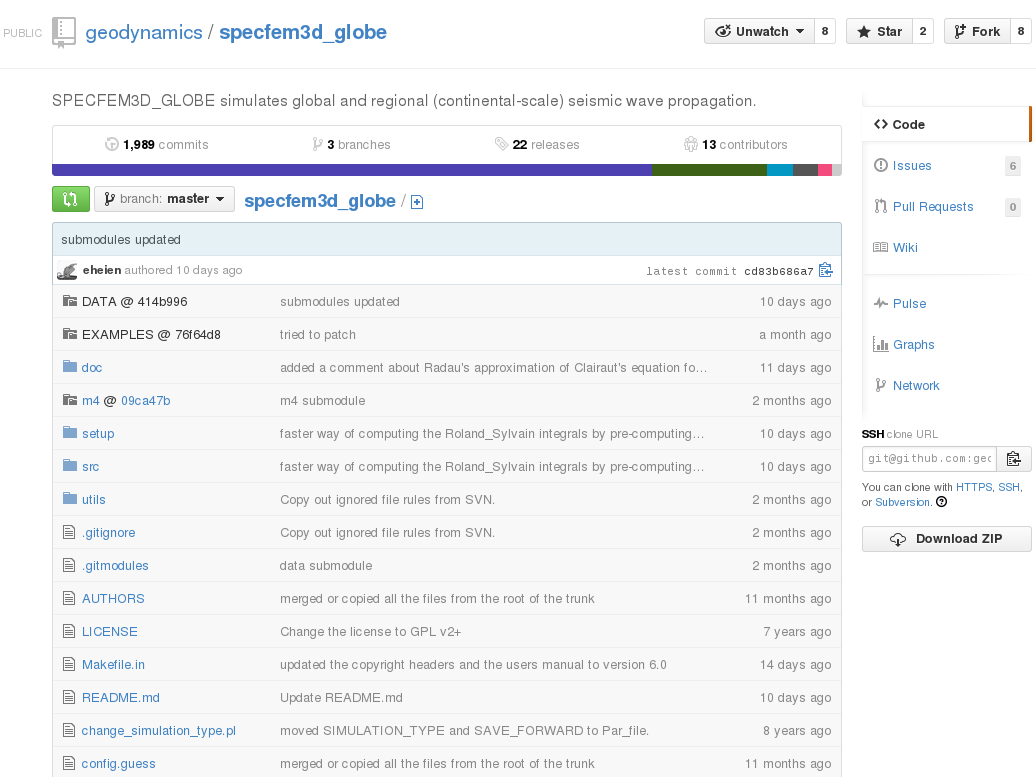
\includegraphics[height=\textheight,width=\textwidth,keepaspectratio]{github}
\end{frame}

\begin{frame}[fragile]
 \frametitle{Using CIG Code from Git}

 \begin{exampleblock}{Cloning Stable Code}
  \begin{semiverbatim}
\command{git clone \alert<2>{-{}-recursive} \\
   https://github.com/geodynamics/specfem3d_globe.git}
Cloning into `specfem3d_globe'...
remote: Reusing existing pack: 20478, done.
remote: Counting objects: 59, done.
remote: Compressing objects: 100% (59/59), done.
done.
Checking out files: 100% (701/701), done.
...
\end{semiverbatim}
 \end{exampleblock}
\end{frame}

\begin{frame}[fragile]
 \frametitle{Using CIG Code from Git}

 \begin{exampleblock}{Cloning Development Code}
  \begin{semiverbatim}
\command{git clone -{}-recursive \alert{-{}-branch devel} \\
   https://github.com/geodynamics/specfem3d_globe.git}
Cloning into `specfem3d_globe'...
remote: Reusing existing pack: 20478, done.
remote: Counting objects: 59, done.
remote: Compressing objects: 100% (59/59), done.
done.
Checking out files: 100% (701/701), done.
...
\end{semiverbatim}
 \end{exampleblock}
\end{frame}

\begin{frame}[fragile]
 \frametitle{Using CIG Code from Git}

 \begin{exampleblock}<only@1>{Switching Branches}
  \begin{semiverbatim}
\comment{Create branch that tracks upstream}
\command{git branch -{}-track devel origin/devel}
Branch origin/devel set up to track local branch \makebox[0.85\width][l]{devel}

\comment{Switch to branch}
\command{git checkout devel}
Switched to branch `devel'
Your branch is up-to-date with `origin/devel'.
\end{semiverbatim}
 \end{exampleblock}

 \begin{exampleblock}<only@2->{Shortcut}
  \begin{semiverbatim}
\comment{Create and switch to branch devel}
\command{git checkout \alert<3>{-{}-track} \alert<2>{-b devel} origin/devel}
Branch origin/devel set up to track local branch \makebox[0.85\width][l]{devel}
Switched to branch `devel'
\end{semiverbatim}
 \end{exampleblock}
\end{frame}

\begin{frame}[fragile]
 \frametitle{Using CIG Code from Git}

 \begin{exampleblock}{Fetching Updates}
  \begin{semiverbatim}
\command{git fetch \only<2>{origin}}
remote: Counting objects: 85, done.
remote: Compressing objects: 100% (85/85), done.
remote: Total 85 (delta 37), reused 2 (delta 0)
Unpacking objects: 100% (85/85), done.
From https://github.com/geodynamics/specfem3d_globe
   c45b60b..f218984  devel      -> origin/devel
\end{semiverbatim}
 \end{exampleblock}
\end{frame}

\begin{frame}[fragile,t]
 \frametitle{Using CIG Code from Git}

 \begin{exampleblock}{Reviewing Updates}
  \begin{semiverbatim}
\comment{Log starting at HEAD}
\command{git log}
\hiYellow{commit 28789049bdcb5d51cbef122842a5e1bf9cd7376d}
Merge: fedf291 2f0c52e
Author: Dimitri Komatitsch <komatits@...>
Date:   Thu May 1 09:48:38 2014 +0200

    Merge pull request \#62 from QuLogic/typos

    Fix some small typos.
\end{semiverbatim}
 \end{exampleblock}
\end{frame}

\begin{frame}[fragile,t]
 \frametitle{Using CIG Code from Git}

 \begin{exampleblock}{Reviewing Updates}
  \vspace{-1em}
  \begin{semiverbatim}
\comment{Log of changes with differences}
\command{git log -{}-patch} \comment{or -p}
\hiYellow{commit 2f0c52e3555c6d534baf40084c5f59f7fd6bc7bc}
Author: Elliott Sales de Andrade <...>
Date:   Wed Apr 30 23:32:33 2014 -0400
    Fix some small typos.
diff --git a/src/auxiliaries/combine_paraview_strain_
index 4c1fe2a..ea6d238 100644
--- a/src/auxiliaries/combine_paraview_strain_data.f9
+++ b/src/auxiliaries/combine_paraview_strain_data.f9
@@ -106,3 +106,3 @@ program combine_paraview_movie_da
\hiRed{-  ! open paraview output mesh file}
\hiGreen{+  ! open Paraview output mesh file}
     write(mesh_file,'(a,a,a,i6.6,a)')  'movie3D_',tr
\end{semiverbatim}
 \end{exampleblock}
\end{frame}

\begin{frame}[fragile,t]
 \frametitle{Using CIG Code from Git}

 \begin{exampleblock}{Reviewing Updates}
  \vspace{-1em}
  \begin{semiverbatim}
\comment{Log of changes with statistics}
\command{git log -{}-stat}
\hiYellow{commit 2f0c52e3555c6d534baf40084c5f59f7fd6bc7bc}
Author: Elliott Sales de Andrade <...>
Date:   Wed Apr 30 23:32:33 2014 -0400
    Fix some small typos.

 src/auxiliaries/combine_surf_data.f90      | 4 \hiGreen{+}\hiRed{-}
 src/auxiliaries/combine_vol_data.F90       |18 \hiGreen{++}\hiRed{-{}-}
 src/auxiliaries/create_movie_AVS_DX.f90    | 6 \hiGreen{+}\hiRed{-}
 src/auxiliaries/create_movie_GMT_global.f90|10 \hiGreen{+}\hiRed{-{}-}
 src/cuda/assemble_MPI_scalar_cuda.cu       |10 \hiGreen{+}\hiRed{-{}-}
 src/cuda/assemble_MPI_vector_cuda.cu       |14 \hiGreen{+}\hiRed{-{}-}
 src/cuda/check_fields_cuda.cu              | 2 \hiGreen{+}\hiRed{-}
\end{semiverbatim}
 \end{exampleblock}
\end{frame}

\begin{frame}[fragile,t]
 \frametitle{Using CIG Code from Git}

 \begin{exampleblock}{Reviewing Updates}
  \begin{semiverbatim}
\comment{Log starting at HEAD -- Short}
\command{git log -{}-oneline}
\hiYellow{2878904} Merge pull request \#62 from QuLogic/typos
\hiYellow{2f0c52e} Fix some small typos.
\hiYellow{fedf291} Merge pull request \#61 from QuLogic/regular-k
\hiYellow{6cea702} Save some memory on addressing array.
\hiYellow{433edf7} Use addressing to find regular grid slices.
\hiYellow{eeeeb36} Round chunk_map output to the nearest EPS.
\hiYellow{672b5e6} Use specfem modules to reduce subroutine argu
\hiYellow{811ae11} Merge pull request \#60 from komatits/devel
\hiYellow{163240c} simpler implementation of volume and area cal
\hiYellow{32686e3} Fix allocation of regular kernel arrays.
\hiYellow{e27d871} Merge pull request \#59 from komatits/devel
\end{semiverbatim}
 \end{exampleblock}
\end{frame}

\begin{frame}[fragile,t]
 \frametitle{Using CIG Code from Git}

 \begin{exampleblock}{Reviewing Updates}
  \begin{semiverbatim}
\comment{Log of new changes}
\command{git log -{}-oneline devel..origin/devel}
\hiYellow{f218984} Merge pull request #88 from komatits/devel
\hiYellow{a5dde6d} added an email from Daniel Peter about ellipt
\hiYellow{f2de2cd} Merge pull request #87 from komatits/devel
\hiYellow{ffd536a} renamed model_crust to model_crust_2_0 to be
\hiYellow{e63245c} Merge pull request #86 from komatits/devel
\hiYellow{2614dd9} done cleaning and adding all the topography
\hiYellow{ba3f67c} Merge pull request #85 from komatits/devel
\hiYellow{04ab1bc} replaced the old version of ETOPO with the
\hiYellow{97da690} Merge pull request #84 from komatits/devel
\hiYellow{85124e8} compressed the large topo files that are
\hiYellow{0e84408} Merge pull request #83 from komatits/devel
\end{semiverbatim}
 \end{exampleblock}
\end{frame}

\begin{frame}[fragile]
 \frametitle{Using CIG Code from Git}

 \begin{exampleblock}{Merge Updates}
  \begin{semiverbatim}
\command{git merge \only<2>{origin/master}}
Updating c45b60b..f218984
Fast-forward
...
\end{semiverbatim}
 \end{exampleblock}
\end{frame}


\section{Local Development}

\begin{frame}[plain,noframenumbering]
 \vfill
 \begin{center}
  \LARGE \color{solarizedAccent} Local Development
 \end{center}
 \vfill
\end{frame}

\begin{frame}
 \frametitle{Local Development}
 \framesubtitle{Forking}

 \begin{itemize}
  \item Push access to Geodynamics repos on GitHub restricted
  \item How to share code?
  \pause
  \item Create a \alert{fork} (personal GitHub copy of repo):
   \begin{tikzpicture}
    \node[anchor=south west, inner sep=0] at (0,0) {
     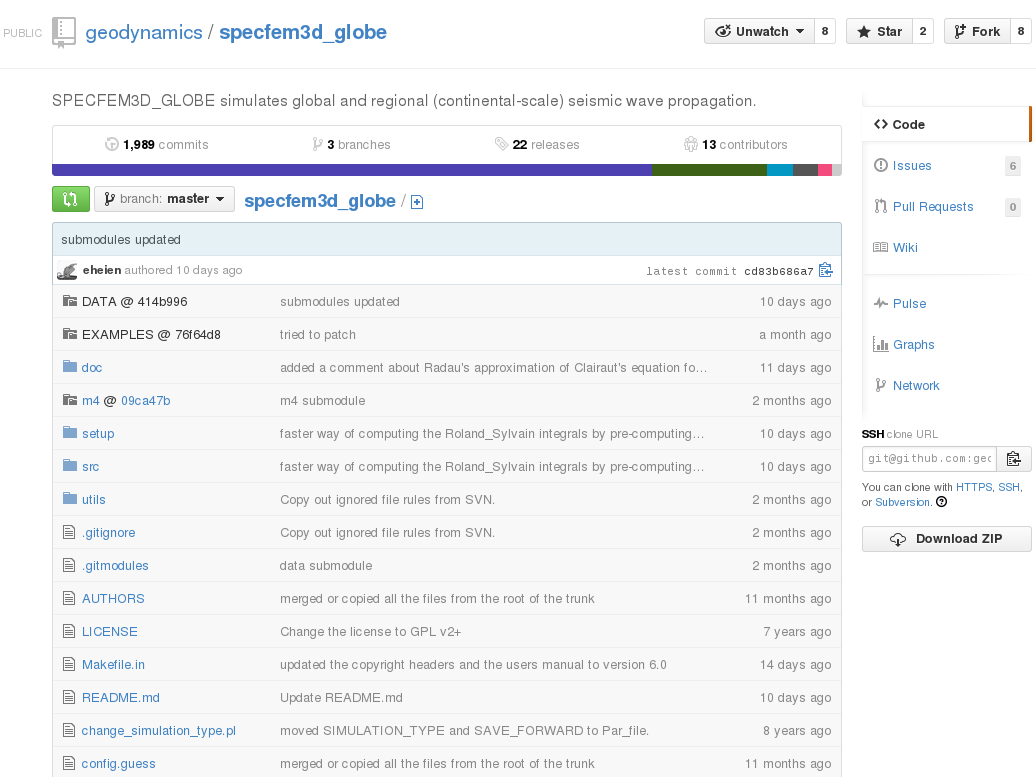
\includegraphics[width=\linewidth, height=\textheight, keepaspectratio,
                      trim={0 700px 0 0}, clip]{github}
    };
    \draw[solarizedAccent, thick, rounded corners]
     (9.1,0.3) rectangle (10.0,0.6);
   \end{tikzpicture}
   \begin{columns}
    \begin{column}{0.4\framewidth}
     \begin{tikzpicture}[
       remember picture,
       show background rectangle,
       commit/.style={draw, rectangle, rounded corners, fill=solarizedRebase02,
                      inner sep=1pt, minimum width=1.5em},
       connections/.style={draw}
      ]
      \matrix [column sep={1em,between origins},
               row sep={1.5em,between origins},
               ampersand replacement=\&]%
      {
       \node[commit] (9) {9}; \\
       \node[commit] (8) {8}; \\
       \node[commit] (7) {7}; \\
       \node[commit] (6) {6}; \\
       \node[commit] (5) {5}; \\
       \ghost{4}; \\
      };
      \node[anchor=south, align=center] (CIG repository) at (9.north)
       {Geodynamics\\Repository};
      \foreach \x in {6,...,9} {
       \pgfmathparse{int(\x-1)}
       \connect{\pgfmathresult}{\x};
      }
      \path[connections, densely dashed] (4) -- (5);
     \end{tikzpicture}
    \end{column}
    \begin{column}{0.3\textwidth}
     \begin{tikzpicture}[
       remember picture,
       show background rectangle,
       commit/.style={draw, rectangle, rounded corners, fill=solarizedRebase02,
                      inner sep=1pt, minimum width=1.5em},
       connections/.style={draw}
      ]
      \matrix [column sep={1em,between origins},
               row sep={1.5em,between origins},
               ampersand replacement=\&]%
      {
       \node[commit] (9) {9}; \\
       \node[commit] (8) {8}; \\
       \node[commit] (7) {7}; \\
       \node[commit] (6) {6}; \\
       \node[commit] (5) {5}; \\
       \ghost{4}; \\
      };
      \node[anchor=south, align=center] (My repository) at (9.north)
       {Personal\\Repository};
      \foreach \x in {6,...,9} {
       \pgfmathparse{int(\x-1)}
       \connect{\pgfmathresult}{\x};
      }
      \path[connections, densely dashed] (4) -- (5);
     \end{tikzpicture}
    \end{column}
   \end{columns}

   \begin{tikzpicture}[
     remember picture, overlay,
     path/.style={thick, ->},
     label/.style={decorate, decoration={text along path, text align=center,
                                         text color=solarizedRebase0,
                                         raise=1pt,
                                         text={Fork}}}
    ]
    \draw[path] (CIG repository) to[out=0,in=180] (My repository);
    \draw[label] (CIG repository) to[out=0,in=180] (My repository);
   \end{tikzpicture}
 \end{itemize}
\end{frame}

\begin{frame}[fragile]
 \frametitle{Local Development}
 \framesubtitle{Forking}

 Set remotes for both repos (conventions):
 \begin{itemize}
  \item \texttt{origin} to your fork
  \item \texttt{upstream} to Geodynamics repo
 \end{itemize}

 \begin{exampleblock}{Setting Remotes}
  \begin{semiverbatim}
\comment{Clone \textit{your} fork}
\command{git clone -{}-recursive \\
   https://github.com/\alert{username}/specfem3d_globe.git}

\comment{Add remote for Geodynamics repo}
\command{git remote add upstream \\
   https://github.com/\alert{geodynamics}/specfem3d_globe.git}
\command{git fetch upstream}
\end{semiverbatim}
 \end{exampleblock}
\end{frame}

\begin{frame}[fragile,t]
 \frametitle{Using CIG Code from Git}
 \framesubtitle{Feature Branches}

 \begin{itemize}
  \item Short-lived branches that contain work on a single feature
  \item Recommended (but not required) development workflow
  \item Completely local (unless explicitly shared)
  \item Allows you to switch between work topics quickly
 \end{itemize}

 \begin{minipage}[t][0.45\textheight][t]{0.97\textwidth}
 \vspace{-1em}
 \begin{exampleblock}<only@1>{Creating a Feature Branch}
  \vspace{-1em}
  \begin{semiverbatim}\small
\comment{Create and switch to branch feature-one}
\command{git checkout -b feature-one devel}
Switched to branch `feature-one'

\comment{Switch back to branch devel}
\command{git checkout devel}
Switched to branch `devel'
\end{semiverbatim}
 \end{exampleblock}

 \begin{exampleblock}<only@2>{Deleting a Feature Branch}
  \vspace{-1em}
  \begin{semiverbatim}\small
\comment{Switch back to branch devel}
\command{git checkout devel}
Switched to branch `devel'

\comment{Delete branch feature-one}
\command{git branch -d feature-one}
Deleted branch feature-one (was 6106a0c).
\end{semiverbatim}
 \end{exampleblock}

 \begin{exampleblock}<only@3>{Listing Branches}
  \vspace{-1em}
  \begin{semiverbatim}\small
\command{git branch}
* \hiGreen{devel}
  master
\end{semiverbatim}
 \end{exampleblock}

 \begin{exampleblock}<only@4>{Listing All Branches (including remotes)}
  \vspace{-1em}
  \begin{semiverbatim}\small
\command{git branch -a}
* \hiGreen{devel}
  master
  \hiRed{remotes/origin/devel}
  \hiRed{remotes/origin/master}
  \hiRed{remotes/upstream/devel}
  \hiRed{remotes/upstream/master}
\end{semiverbatim}
 \end{exampleblock}
 \end{minipage}
\end{frame}

\begin{frame}[fragile]
 \frametitle{Local Development}
 \framesubtitle{Reviewing Changes}

 \begin{exampleblock}{Checking Status}
  \vspace{-1em}
  \begin{semiverbatim}
\command{git status}
On branch devel

Changes not staged for commit:
  (use "git add <file>..." to update what will be
   committed)
  (use "git checkout -{}- <file>..." to discard changes
   in working directory)
    \hiRed{modified:   DATA} (new commits)
    \hiRed{modified:   src/specfem3D/specfem3D.F90}

no changes added to commit (use "git add" and/or "git
commit -a")
\end{semiverbatim}
 \end{exampleblock}
\end{frame}

\begin{frame}[fragile]
 \frametitle{Local Development}
 \framesubtitle{Reviewing Changes}

 \begin{exampleblock}{Viewing Diffs}
  \vspace{-1em}
  \begin{semiverbatim}
\command{git diff \only<2->{master} \only<3>{-{}- src/}}\uncover<3>{
\textbf{\color{solarizedBase1}diff -{}-git a/src/specfem3D/specfem3D.F90 b/src/..
index 3ba52f2..2b619bf 100644
-{}-{}- a/src/specfem3D/specfem3D.F90
+++ b/src/specfem3D/specfem3D.F90}
\hiBlue{ @@ -466,6 +466,6 @@}
   ! sets up and precomputes simulation arrays
   call prepare_timerun()

\hiRed{-  ! steps through time iterations}
\hiGreen{+  ! Test change}
   if( UNDO_ATTENUATION ) then
     call iterate_time_undoatt()}
\end{semiverbatim}
 \end{exampleblock}
\end{frame}

\begin{frame}
 \frametitle{Local Development}
 \framesubtitle{Working with the Index}

 \begin{itemize}
  \item \alert{Index} or \alert{staging area} stores changes to be committed

  \begin{tikzpicture}[%
    remember picture,
    show background rectangle,
    background rectangle/.style={draw, visible on=<2->},
    visible on=<2->
   ]
   \begin{scope}[
     commit/.style={draw, rectangle, rounded corners, fill=solarizedRebase02,
                    inner sep=1pt, minimum height=0.75em, minimum width=1em,
                    font={\tiny\sffamily}},
     connections/.style={draw}
    ]
    \matrix [column sep={1em,between origins}, row sep={1em,between origins},
             ampersand replacement=\&]%
    {
     \node[commit,visible on=<5->] (10) {\alert<5>{10}}; \\
     \node[commit] (9) {9}; \\
     \node[commit] (8) {8}; \\
     \node[commit] (7) {7}; \\
     \node[commit] (6) {6}; \\
     \node[commit] (5) {5}; \\
     \ghost{4}; \\
    };
    \node[anchor=south, align=center, font={\scriptsize}] at (10.north)
     (repository) {Local\\Repository};
    \foreach \x in {6,...,9} {
     \pgfmathparse{int(\x-1)}
     \connect{\pgfmathresult}{\x};
    }
    \path[connections, densely dotted] (4) -- (5);
    \path[connections, visible on=<5->] (9) -- (10);
   \end{scope}
   \begin{scope}[
     every node/.style={anchor=west, minimum height=1em,
                        font={\tiny\ttfamily}, inner sep=2.5pt},
     every edge/.style={thick},
     root/.style={},
     grow via three points={one child at (0.25,-0.75em) and
                            two children at (0.25,-0.75em) and (0.25,-1.25em)},
     edge from parent path={(\tikzparentnode.south) |- (\tikzchildnode.west)}
    ]
    \node[anchor=west, font={\scriptsize\sffamily}, align=center, xshift=3em]
     at (repository.east) (index) {Index};
    \node [root, anchor=north, visible on=<4-5>] at (index.south) (index root)
     {src};
   \end{scope}
   \begin{scope}[
     every node/.style={anchor=west, minimum height=1em,
                        font={\tiny\ttfamily}, inner sep=2.5pt},
     every edge/.style={thick},
     root/.style={},
     grow via three points={one child at (0.25,-0.75em) and
                            two children at (0.25,-0.75em) and (0.25,-1.25em)},
     edge from parent path={(\tikzparentnode.south) |- (\tikzchildnode.west)}
    ]
    \node[anchor=west, font={\scriptsize\sffamily}, align=center, xshift=3em]
     at (index.east) (work) {Working\\Directory};
    \node [root, anchor=north] at (work.south) (work root) {specfem3d\_globe}
     child { node {DATA} }
     child { node {doc} }
     child { node {EXAMPLES} }
     child { node {setup} }
     child { node (work src) {\alert<3-4>{src}} }
     child { node {utils} }
     child { node {\dots} };
   \end{scope}
   \node[anchor=south, shift={(0em,1em)}] at (index.north)
    {Information Flow};

   \begin{scope}[
     path/.style={->},
     label/.style={decorate, decoration={text along path, text align=center,
                                         text color=solarizedRebase0,
                                         raise=1pt}}
    ]
    \draw<2>[path] (9.east) to[out=0,in=180] (work root.west);
    \draw<2>[label, decoration={text={|\tiny| git checkout}}]
     (9.east) to[out=0,in=180] (work root.west);
    \draw<4>[path] (work src.west) to[out=180,in=0] (index root.east);
    \draw<4>[label, decoration={text={|\tiny| git add}}]
     (index root.east) to[out=0,in=180] (work src.west);
    \draw<5>[path] (index root.west) to[out=180,in=0] (10.east);
    \draw<5>[label, decoration={text={|\scriptsize| git commit}}]
     (10.east) to[out=0,in=180] (index root.west);
    \draw<6->[dashed] (work root.west) to[out=180,in=0] (10.east);
   \end{scope}
  \end{tikzpicture}
  \item<7-> Option \texttt{-{}-cached} makes commands work in reference to index
  \begin{itemize}
   \item \texttt{git diff} compares index with working directory
   \item \texttt{git diff -{}-cached} compares HEAD with index
  \end{itemize}
 \end{itemize}
\end{frame}

\begin{frame}[fragile]
 \frametitle{Local Development}
 \framesubtitle{Working with the Index}

 \begin{exampleblock}{Adding New Files}
  \begin{semiverbatim}
\command{git add <new file>}
\end{semiverbatim}
 \end{exampleblock}

 \begin{exampleblock}<2->{Removing \textit{Existing} Files}
  \begin{semiverbatim}
\command{git rm <file>}
\end{semiverbatim}
 \end{exampleblock}

 \begin{exampleblock}<3>{Removing \textit{Newly Added} Files (i.e., from index)}
  \begin{semiverbatim}
\command{git rm -{}-cached <file>}
\end{semiverbatim}
 \end{exampleblock}
\end{frame}

\begin{frame}[fragile]
 \frametitle{Local Development}
 \framesubtitle{Working with the Index}

 \begin{exampleblock}{Adding Changes in Files}
  \begin{semiverbatim}
\comment{Add changes from file, patch-by-patch}
\command{git add -{}-patch} \comment{or -p}
\pause
\comment{Add entire change of file (not recommended)}
\command{git add <modified file>}
\pause
\comment{Add all changes of{\em tracked} files (not recommended)}
\command{git add -{}-all}
\end{semiverbatim}
 \end{exampleblock}
\end{frame}

\begin{frame}[fragile]
 \frametitle{Local Development}
 \framesubtitle{Working with the Index}

 \begin{exampleblock}{Undo Changes to Files}
  \begin{semiverbatim}
\comment{Remove changes to files}
\comment{(will match index)}
\command{git checkout -{}- <files>}
\pause
\comment{Remove changes from index}
\comment{(working directory unaltered)}
\command{git reset \uncover<3->{-{}- <files>}}
\pause\pause
\comment{Remove changes from files{\em and} index}
\command{git reset -{}-hard}
\end{semiverbatim}
 \end{exampleblock}
\end{frame}

\begin{frame}[fragile]
 \frametitle{Local Development}
 \framesubtitle{Committing}

 \begin{exampleblock}{Committing Changes in Index}
  \begin{semiverbatim}
\command{git commit}
\end{semiverbatim}
 \end{exampleblock}

 \begin{block}{Commit Messages}
\begin{verbatim}
Capitalized, short (50 chars or less) summary

More detailed explanatory text, if necessary.  Wrap
it to about 72 characters or so.  The blank line
separating the summary from the body is critical
(unless you omit the body entirely); tools like
rebase can get confused if you run the two together.
\end{verbatim}
 \end{block}
\end{frame}

\begin{frame}[fragile,t]
 \frametitle{Using CIG Code from Git}

 \begin{itemize}
  \item Merging may cause \alert{conflicts} --- when upstream changes lines you
        have also changed
  \item Produces conflict markers \alert{<{}<{}<===>{}>{}>} in conflicting files
  \item Status shows conflicting files
  \item Must be added to index to resolve conflict
 \end{itemize}

 \begin{minipage}[t][0.5\textheight][t]{0.97\textwidth}
  \begin{exampleblock}<only@1>{Conflict Status\textcolor{solarizedRebase02}{g}}
   \begin{semiverbatim}
\command{git status}
...
 Unmerged paths:
    (use "git add ..." to mark resolution)

  \hiRed{both modified:   src/specfem3D/specfem3D.F90}
\end{semiverbatim}
  \end{exampleblock}

  \begin{exampleblock}<only@2->{Resolving Conflicts}
   \begin{semiverbatim}
\command{git mergetool \only<3->{-{}-tool=meld}}

\only<4>{\comment{Permanent tool setting}}
\only<4>{\command{git config -{}-global merge.tool meld}}
\end{semiverbatim}
  \end{exampleblock}
 \end{minipage}
\end{frame}

\begin{frame}
 \frametitle{Submodules (or, ``Why git clone -{}-recursive?'')}

 \begin{itemize}
  \item Completely \alert{independent} repositories referenced in another
  \item Changes, commits, etc.{} are local to submodule
  \item Parent just sees a \textit{single} directory --- always treat it as such
  \item \texttt{git fetch} in parent will automatically fetch submodules
  \item \texttt{git fetch} in submodule will \textit{not} fetch parent
  \item \texttt{git submodule update} to keep submodule in sync with parent
 \end{itemize}
\end{frame}


\section{Contributing Code}

\section{Additional Information}

\begin{frame}
 \frametitle{Additional Information}

 \begin{itemize}
  \item \href{http://www.vogella.com/tutorials/Git/article.html}{\textit{Git - Tutorial}}
   by Lars Vogel
  \item \href{http://www.git-tower.com/blog/git-cheat-sheet/}{\textit{Git Cheat Sheet}}
  \item \href{https://github.com/geodynamics/specfem3d/wiki/Git-tips-for-developers}{\textit{Git tips for developers}}
   on Specfem3D wiki
  \item \href{http://git-scm.com/book}{\textit{Pro Git book}}
  \item \href{https://try.github.io/levels/1/challenges/1}{\textit{Try Git}}
   in your browser
 \end{itemize}
\end{frame}

\end{document}
